\section{内存管理}

内存 (RAM) 是计算机中不可缺少的重要硬件,所有程序的运行都是在内存中进行的,
而CPU访问硬盘数据也必须先经过内存交换才得以实现,内存在加速CPU访问硬盘居功至伟。
由内存的重要性可知内存管理在操作系统中也非常重要。	

根据内存的特殊性,内存错误将导致程序或操作系统错误,
故操作系统将在内存管理中首先检测内存是否故障,
确认内存完好后开始对内存进行初始化并清空内存空间内容,在程序申请内存后向其分配内存,
并程序运行结束后释放其内存。功能设计如图~\ref{fig:memman}。
\begin{figure}[H]
  \centering
  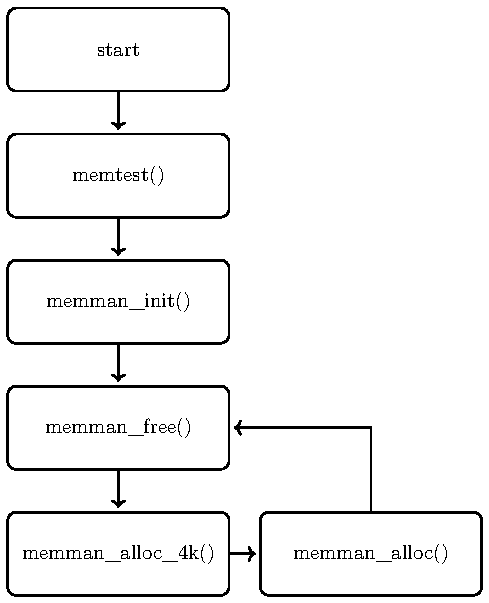
\includegraphics[width=.5\textwidth]{../Fig/func/memman.pdf}
  \caption{内存管理}
  \label{fig:memman}
\end{figure}

\csingle|unsigned int memtest(unsigned int start, unsigned int end);|
\begin{itemize}
  \item 检测整个内存并返回可用内存大小;
\end{itemize}

\csingle|void memman_init(struct MEMMAN *man);|
\begin{itemize}
  \item 初始化各内存块,并初始化块信息;
\end{itemize}

\csingle|int memman_free(struct MEMMAN *man, unsigned int addr, unsigned int size);|
\begin{itemize}
  \item 释放指定大小的内存地址空间;
\end{itemize}

\csingle|unsigned int memman_alloc_4k(struct MEMMAN *man, unsigned int size);|
\begin{itemize}
  \item 分配指定大小的内存空间;\\
\end{itemize}

内存的结构通常用地址和空间表示,在计算机运行过程中,
内存的分配是随机的,导致内存的释放也是相对无序的,这样导致了很多的碎片化问题,
也就是随计算机运行时间变长,内存中到处遍布小块零散空闲空间,虽然零散空间总数很大,
但很难满足新进程序的内存需求,于是内存管理显得十分必要。

内存管理设计的主要目的是快速并且高效的分配内存空间,并在适当的时间释放并回收内存空间。
根据内存管理的设计目的,数据结构设计如程序~\ref{lst:mem}。

\begin{listing}[H]
  \inputminted[tabsize=2, firstline=137, lastline=143,
    linenos=true]{c}{../ZOS/src/kernel/bootpack.h}
  \caption{数据结构-内存管理}
  \label{lst:mem}
\end{listing}

\begin{description}
\item[frees:]当前可用内存组数;
\item[maxfrees:]可用内存组数的最大;
\item[lostsize:]释放失败的内存的大小总和;
\item[losts:]释放失败次数。
\end{description}

经过内存初始化和释放所有内存空间后,内存管理正常运行。

\subsection{内存分配}

内存的分配方式涉及到内存释放,好的分配方式会使得内存使用的效率大大提高。
根据内存的大小来划分内存如何使用,预计使用32KB用于内存分配的管理空间,
则共有4000组左右的内存用于分配给各个程序使用,每个组4KB。

每一组内存经过初始化都拥有自己的数据结构,
即每一组空闲内存的地址和大小都被记录到空闲内存表,如表~\ref{tab:free}。

\begin{table}[h]
  \centering
  \begin{tabular}{cc}
    \hline
    组号 & 地址 \\\hline
    2 & 0x00005000 \\ 
    1 & 0x00004000 \\
    0 & 0x00003000 \\\hline    
  \end{tabular}
  \caption{空闲内存表free}
  \label{tab:free}
\end{table}

一旦系统接收到程序申请内存的请求(需求的内存大小),
就开始在内存中寻找足够大的内存完成这次申请,并返回可供使用的空闲内存的地址。
完成申请后系统需要重新整理空闲内存表free,将可用内存组数减一,
将返回给程序空闲空间大小根据程序需求进行调整,并对剩余的可用内存表进行按地址升序整理。
流程见图~\ref{fig:memman},实现见程序~\ref{lst:alloc}。

% ----------------------------

\subsection{内存释放}

为保证磁盘空闲空间尽可能少的碎片化,内存释放首先考虑的是使待释放空间与附近空闲空间进行合并\cite{bryant2003computer}。

具体分为三种情况:

\begin{description}
\item[前端空闲:]释放内存的相连前端是空闲内存或释放内存相连两端都是空闲内存;
\item[后端可用:]释放内存的相连后端是空闲空间;
\item[前端后端均不可用:]在当前位置释放内存。
\end{description}

已知:待释放的空间的地址和空间大小。

根据空闲内存表free的编号从0到frees遍历查找地址大于待释放空间的空闲内存,
并根据得到的空闲内存编号i及大小size区分此时的待释放内存应当采取何种方式释放,实现参见附录程序~\ref{lst:rw}。

\newpage
前端空闲:

当相连前端有可用内存时,将可释放内存大小归入前端可用内存内,frees不变;

当相连后端也有可用内存时,将后端内存大小归入前端可用内存内,frees减一。

内存释放前后情况如图~\ref{fig:mem0}和图~\ref{fig:mem1}所示,实现见附录程序~\ref{lst:mem1}: 

\begin{figure}[h]
  \centering
  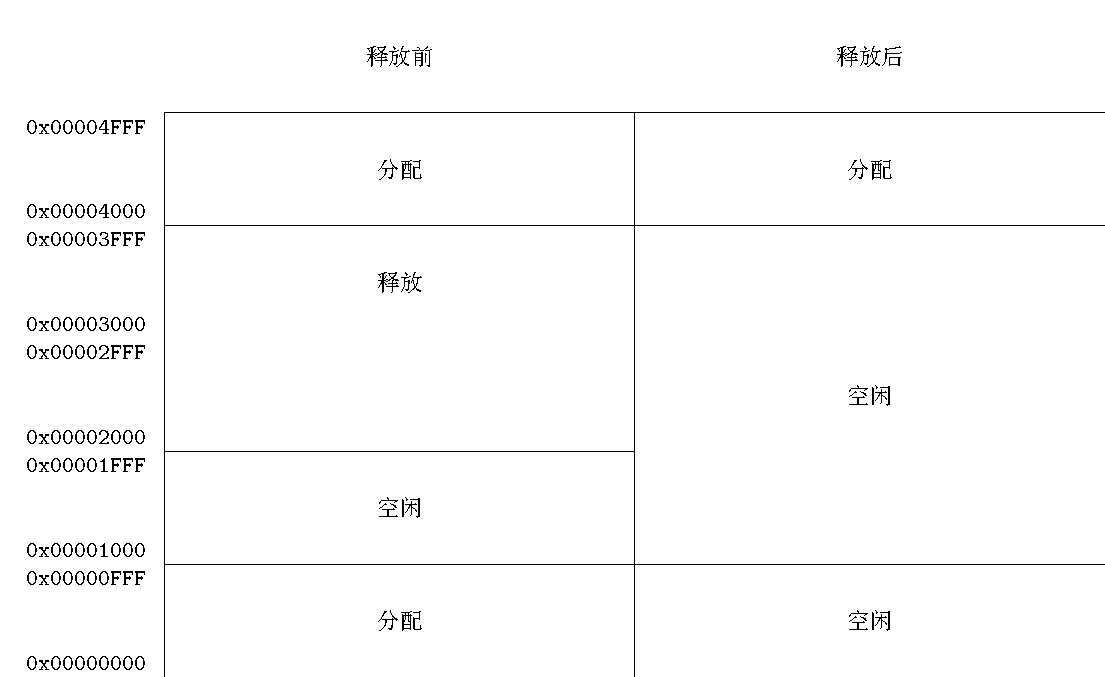
\includegraphics[width=.7\textwidth]{../Fig/mem0.pdf}
  \caption{前端空闲}
  \label{fig:mem0}
\end{figure}

\begin{figure}[h]
  \centering
  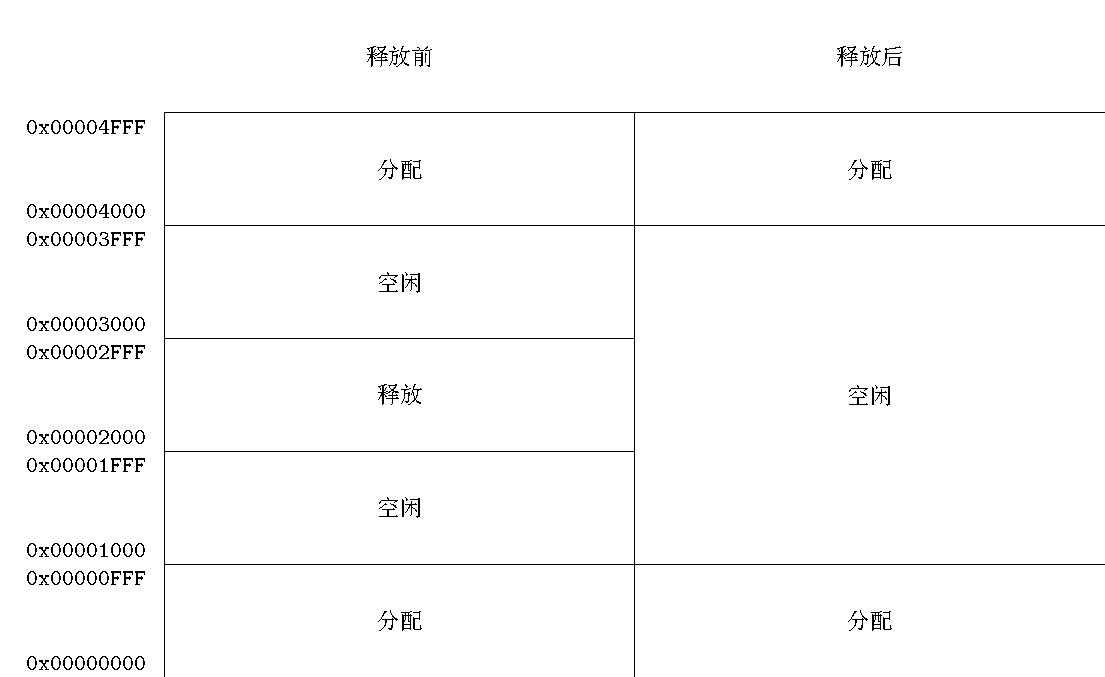
\includegraphics[width=.7\textwidth]{../Fig/mem1.pdf}
  \caption{前端可用,且后端空闲}
  \label{fig:mem1}
\end{figure}

% ------------------------------

\newpage
后端空闲:

当相连后端有可用内存的时候将free[i]的地址换为待释放内存的地址,相连后端内存大小归入待释放内存大小,frees不变。

内存释放前后情况如图~\ref{fig:mem2}所示,实现见附录程序~\ref{lst:mem2}。

\begin{figure}[h]
  \centering
  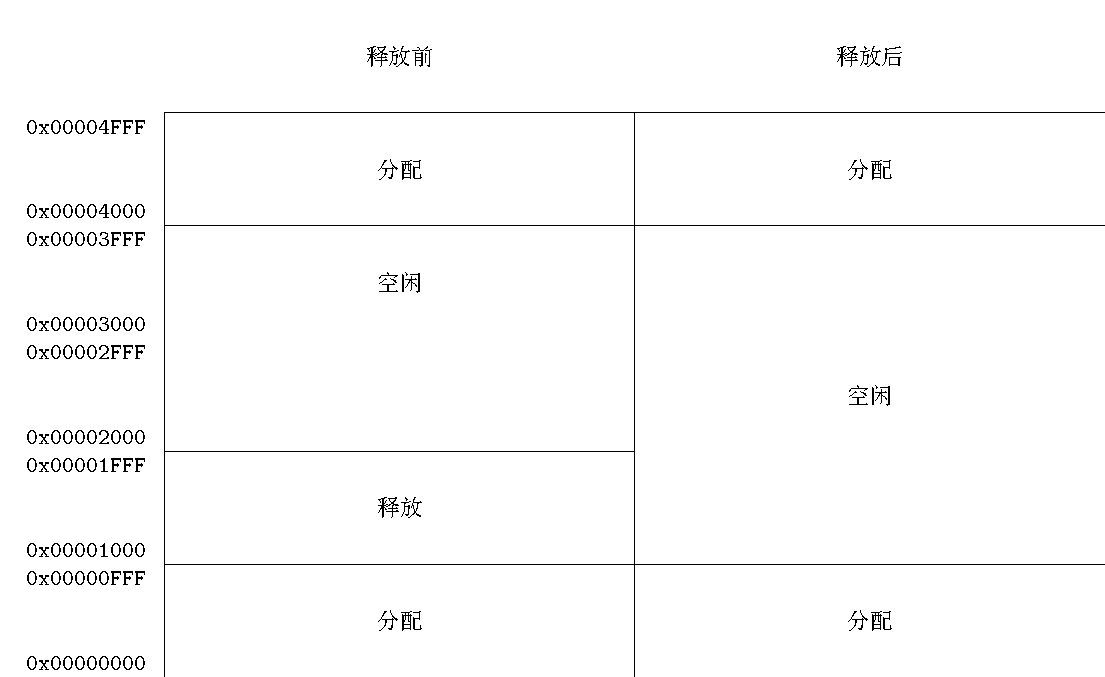
\includegraphics[width=.7\textwidth]{../Fig/mem2.pdf}
  \caption{后端空闲}
  \label{fig:mem2}
\end{figure}

% -----------------------------

前端后端均被占用:

由于被释放空间周围没有空闲内存,为保证free内各段内存仍然按照内存地址升序排列,
使空闲空间计数最大值加一,free[i]后续空闲内存序号加一,并将释放空间组号定为i。

内存释放前后情况如图~\ref{fig:mem3}所示,实现见附录程序~\ref{lst:mem3}。
\begin{figure}[h]
  \centering
  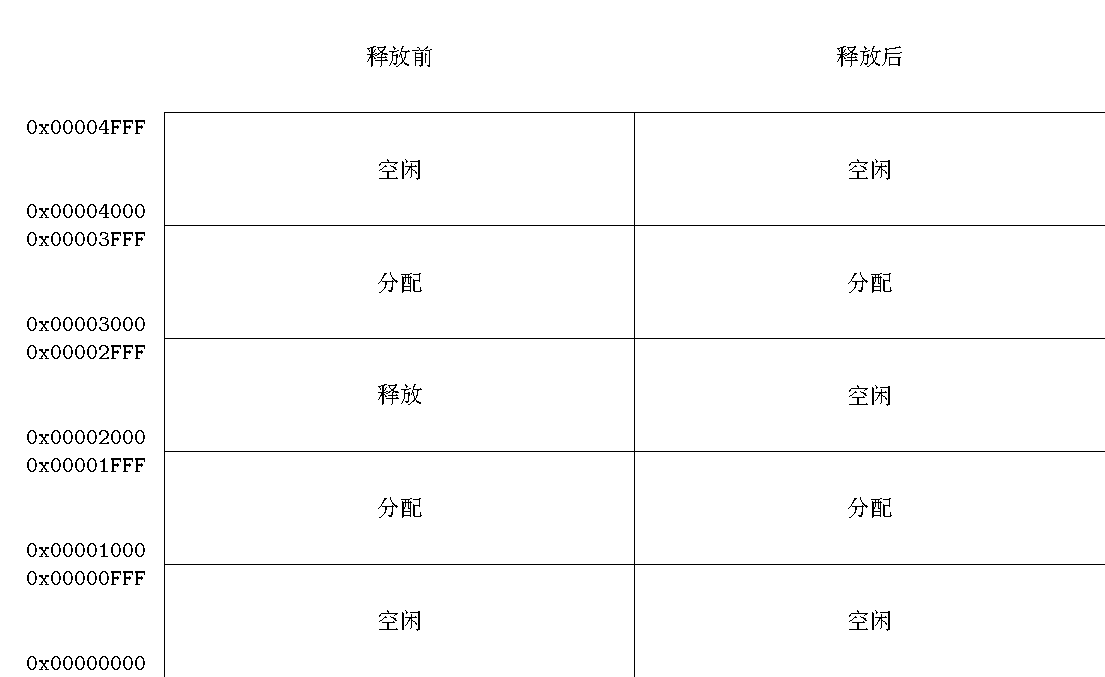
\includegraphics[width=.7\textwidth]{../Fig/mem3.pdf}
  \caption{前端后端均被占用}
  \label{fig:mem3}
\end{figure}